\documentclass[conference]{IEEEtran}
\usepackage[utf8]{inputenc}
\usepackage[T1]{fontenc}
\usepackage[french]{babel}
\usepackage{amsmath,amssymb}
\usepackage{graphicx}
\usepackage{cite}
\usepackage{url}
\usepackage{booktabs}
\usepackage{hyperref}

\begin{document}

\title{Optimisation multiobjectif de l'authentification et de la gestion des clés adaptée au contexte pour les réseaux IoT LoRa~:\\
étude de cas face à un schéma publié d'authentification hybride empreinte radio / MAC}

\author{
\IEEEauthorblockN{Parfait Deffohe}
\IEEEauthorblockA{Master 2 Intelligence Artificielle et Robotique (IAR)\\
CY Cergy Paris Universit\'e\\
Cergy, France}
\and
\IEEEauthorblockN{Lylia Alouache}
\IEEEauthorblockA{Laboratoire ETIS, UMR 8051\\
CY Cergy Paris Universit\'e\\
Cergy, France\\
lylia.alouache@cyu.fr}
\and
\IEEEauthorblockN{Victor Mollimard}
\IEEEauthorblockA{Laboratoire ETIS, UMR 8051\\
CY Cergy Paris Universit\'e\\
Cergy, France\\
victor.mollimard@cyu.fr}
}

\maketitle

\begin{abstract}
Les capteurs LoRa alimentés par batterie doivent choisir, pour chaque message, une méthode d'authentification et une méthode de gestion de clé. L'empreinte radiofréquence (RFF) coûte peu en énergie mais n'est pas parfaite, et les codes d'authentification de message (MAC) cryptographiques sont fiables mais coûteux. Un schéma hybride publié par Haenel et al.\ (Sensors, 2021) replie du RFF vers un MAC selon une règle fixe. Dans ce travail, un arbitre de décision multiobjectif (P0) est proposé à la place. P0 filtre les options admissibles, construit leur front de Pareto et sélectionne une option par scalarisation de Tchebycheff, sous un plancher explicite de fausse acceptation. Chaque comparaison est présentée avec sa référence. Sur cinq scénarios adaptatifs, P0 n'accepte aucune des 4\,426 à 54\,131 tentatives de l'attaquant par scénario, alors qu'une politique physique naïve sans plancher de fausse acceptation (B2) en accepte 12,6\,\% (S2), 55,2\,\% (S5) et 70,6\,\% (S4). Face à la politique conventionnelle toujours cryptographique (B1), P0 économise 2,8\,\% (S1) et 6,9\,\% (S5) d'énergie, et l'économie est inférieure à 0,1\,\% en S2 à S4. Face à une règle hybride fixe (B3), P0 sert toutes les requêtes, alors que B3 en sert entre 0,05\,\% et 44,1\,\% en S2 à S5. Face à l'énergie publiée par Haenel et al.\ (FRR=10\,\%, Tableau~I), P0 consomme 24,4\,\% d'énergie de plus à poids égaux. Ce choix se situe sur une égalité exacte qu'un déplacement de poids de 0,001 suffit à inverser. Les valeurs d'énergie sont calibrées et non mesurées, et tous les résultats proviennent de simulations.
\end{abstract}

\begin{IEEEkeywords}
Sécurité IoT, empreinte radiofréquence, authentification de couche physique, décision multiobjectif, authentification économe en énergie, optimalité de Pareto, scalarisation de Tchebycheff.
\end{IEEEkeywords}

\section{Introduction}

Les capteurs IoT alimentés par batterie doivent authentifier chaque message en dépensant le moins d'énergie possible. Les codes d'authentification de message (MAC) cryptographiques offrent une garantie de sécurité bien comprise, mais ils consomment des cycles CPU et, dans une variante défi-réponse, un aller-retour radio supplémentaire. L'empreinte radiofréquence de couche physique (RFF) authentifie un message presque sans coût énergétique, en exploitant les imperfections analogiques de l'émetteur. Elle présente néanmoins un taux de faux rejet (FRR) et un taux de fausse acceptation (FAR) qui ne peuvent pas être ramenés à zéro.

Les schémas hybrides combinent les deux mécanismes. Haenel et al.~\cite{haenel2021practical} tentent d'abord le RFF et ne replient vers un MAC que lorsque l'empreinte est rejetée. L'énergie consommée par ce repli est mesurée sur une plateforme réelle MSP430G2x et CC110L, tandis que le FAR de l'étape RFF est mesuré séparément. La règle de repli reste fixe et ne pondère pas l'énergie, la latence, la robustesse et la qualité de clé les unes par rapport aux autres.

Une règle fixe de ce type n'est qu'un point d'un espace de conception plus vaste. Un arbitre général pourrait choisir, à chaque période, parmi les options d'authentification et de gestion de clé disponibles, selon des préférences explicites. L'arbitre étudié ici est appelé P0. Les contributions de ce travail sont les suivantes~:
\begin{itemize}
  \item une transposition calibrée des valeurs d'énergie publiées par Haenel et al., dans laquelle le FAR publié du RFF, et non le FAR d'un modèle de canal interne, est fourni à l'arbitre~;
  \item une caractérisation analytique et numérique du cas à deux candidats, montrant que la décision à poids égaux est une égalité exacte de scalarisation, inversée par un déplacement de poids de 0,001~;
  \item une comparaison de P0 avec quatre politiques de référence sur cinq scénarios, fondée sur des nombres aléatoires communs, des statistiques appariées et une correction documentée de la scalarisation~;
  \item un bilan explicite des limites de l'étude, incluant l'incertitude de la calibration énergétique et la part du surcoût de repli qu'un modèle ascendant n'explique pas (de 0,19\,\% à 14,45\,\% du surcoût incrémental).
\end{itemize}

\section{État de l'art et positionnement}
\label{sec:related}

\textbf{Classifieurs d'empreinte RF.} L'identification par empreinte RF a été étudiée en profondeur à l'aide de classifieurs neuronaux et de traitements du signal. Des réseaux profonds et récurrents ont été entraînés sur des signaux IoT bruts~\cite{das2018deep,merchant2019enhanced}. Des réseaux à valeurs complexes et le filtrage adapté ont été utilisés pour améliorer la robustesse au canal et au décalage de fréquence porteuse~\cite{gopalakrishnan2019robust,wilson2019integration}. Des approches fondées sur l'entropie et sur la radio logicielle ont été proposées pour des dispositifs contraints~\cite{baldini2017physical,nouichi2019iot}, et une méthode d'empreinte propre, à faible complexité, a récemment été conçue pour l'IoT~\cite{morge2022rf}. Ces travaux optimisent la précision de l'empreinte. Ils ne décident pas quand un résultat RFF doit être préféré à une vérification cryptographique, et ils ne chiffrent pas cette décision en énergie.

\textbf{Authentification hybride RFF/MAC.} Le travail le plus proche de la présente étude est celui de Haenel et al.~\cite{haenel2021practical}. Ses mesures d'énergie sont retenues comme référence commune, car elles constituent, à la connaissance de la littérature examinée, les seules données publiées pour ce schéma hybride sur matériel contraint. Ce travail présente deux limites. D'une part, la règle de repli est fixe et ne s'adapte pas au contexte. D'autre part, le FAR de l'étape RFF est mesuré dans une expérience de classification qui n'est pas couplée au banc d'essai énergétique. Les deux résultats ne sont reliés que par un FRR de 10\,\%, choisi explicitement pour correspondre à ce FAR. Aucun FAR n'est rapporté pour la configuration à FRR de 5\,\%.

\textbf{Authentification cryptographique économe en énergie.} Du côté cryptographique, des protocoles légers fondés sur des MAC ont été optimisés pour l'IoT industriel contraint en énergie~\cite{li2018robust}. Ces travaux améliorent le coût d'un seul mécanisme. Ils ne sélectionnent pas entre mécanismes et ne représentent pas l'option de couche physique.

\textbf{Sélection multiobjectif de mécanismes de sécurité.} L'optimisation multiobjectif a été utilisée pour recommander des schémas de communication de groupe sécurisés selon des objectifs concurrents de coût et de sécurité~\cite{prantl2023recommendation}. Plus récemment, des protocoles cryptographiques légers et de construction de topologie pour réseaux de capteurs sans fil ont été classés sous contraintes énergétiques~\cite{prvulovic2025hermees}. Ces travaux montrent que la sélection de mécanismes de sécurité est un problème multiobjectif reconnu. Leurs candidats sont toutefois des protocoles fixes évalués une seule fois, sans option de couche physique, et un plancher de fausse acceptation n'y est pas traité comme une contrainte dure.

\textbf{Lacune et positionnement.} Sur la base des travaux examinés ci-dessus, aucune étude antérieure ne combine (i) la sélection, à chaque période, entre une option de couche physique et des options cryptographiques, (ii) l'application d'un plancher de fausse acceptation, (iii) le choix de la gestion de clé et (iv) la comparaison avec une référence énergétique publiée, à mêmes performances de sécurité. Cette lacune est traitée par la présente étude. La décision scalarisée de P0 est retenue comme objet d'analyse, car son comportement peut être caractérisé exactement dans le cas réduit et testé dans le cadre à cinq scénarios. Une base fondée sur la règle fixe et une base conventionnelle sont conservées pour la comparaison.

\section{Contexte}
\label{sec:background}

\subsection{Schéma hybride de Haenel et al.}

Chaque message est d'abord authentifié par RFF. Lorsque le test d'empreinte rejette le message, un échange défi-réponse par MAC (Chaskey-12) est déclenché. Le banc d'essai énergétique émet un message toutes les 3~s pendant 300~s, soit 100 messages, sur un microcontrôleur MSP430G2x associé à un émetteur CC110L. L'énergie est mesurée avec EnergyTrace. Le tableau~\ref{tab:published} présente les quatre valeurs d'énergie publiées. Haenel et al.\ rapportent aussi que le protocole hybride consomme un peu plus au démarrage, en raison d'une authentification complète initiale, avant que le chemin RFF ne devienne moins coûteux après environ six transmissions. Cet effet est décrit qualitativement, sans être quantifié.

\begin{table}[t]
\centering
\caption{Mesures d'énergie publiées (Haenel et al., Tableau 1).}
\label{tab:published}
\begin{tabular}{lc}
\toprule
Configuration & Énergie sur 300~s (mJ) \\
\midrule
RFF seul (théorique, sans repli) & 355,412 \\
Hybride, FRR $=5\%$ & 404,790 \\
Hybride, FRR $=10\%$ & 454,076 \\
MAC seul & 564,743 \\
\bottomrule
\end{tabular}
\end{table}

\subsection{Arbitre de décision P0}

P0 évalue un ensemble de candidats, chacun combinant une méthode d'authentification et une méthode de gestion de clé. Les candidats sont filtrés par des règles d'admissibilité. Les candidats admissibles sont ensuite placés sur un front de Pareto selon quatre objectifs~: énergie attendue, latence normalisée, robustesse d'authentification ($1-$ probabilité totale de fausse acceptation) et qualité de gestion de clé. Le candidat retenu minimise une distance de Tchebycheff pondérée au point idéal,
\begin{equation}
  s(\mathbf{d}) = \max_k \; w_k \cdot
  \frac{f_k(\mathbf{d}) - f_k^{\mathrm{ideal}}}{f_k^{\mathrm{nadir}} - f_k^{\mathrm{ideal}}},
  \label{eq:tcheby}
\end{equation}
où $w_k$ est le poids de l'objectif $k$. Les égalités, à une tolérance près, sont départagées par FAR croissant, puis par énergie, puis par latence, et enfin par un ordre lexicographique des actions. Un plancher de FAR est appliqué avant la scalarisation~: un candidat dont la probabilité totale de fausse acceptation dépasse ce plancher n'est pas admissible. Le modèle de décision est résumé à la figure~\ref{fig:model}.

\begin{figure}[t]
\centering
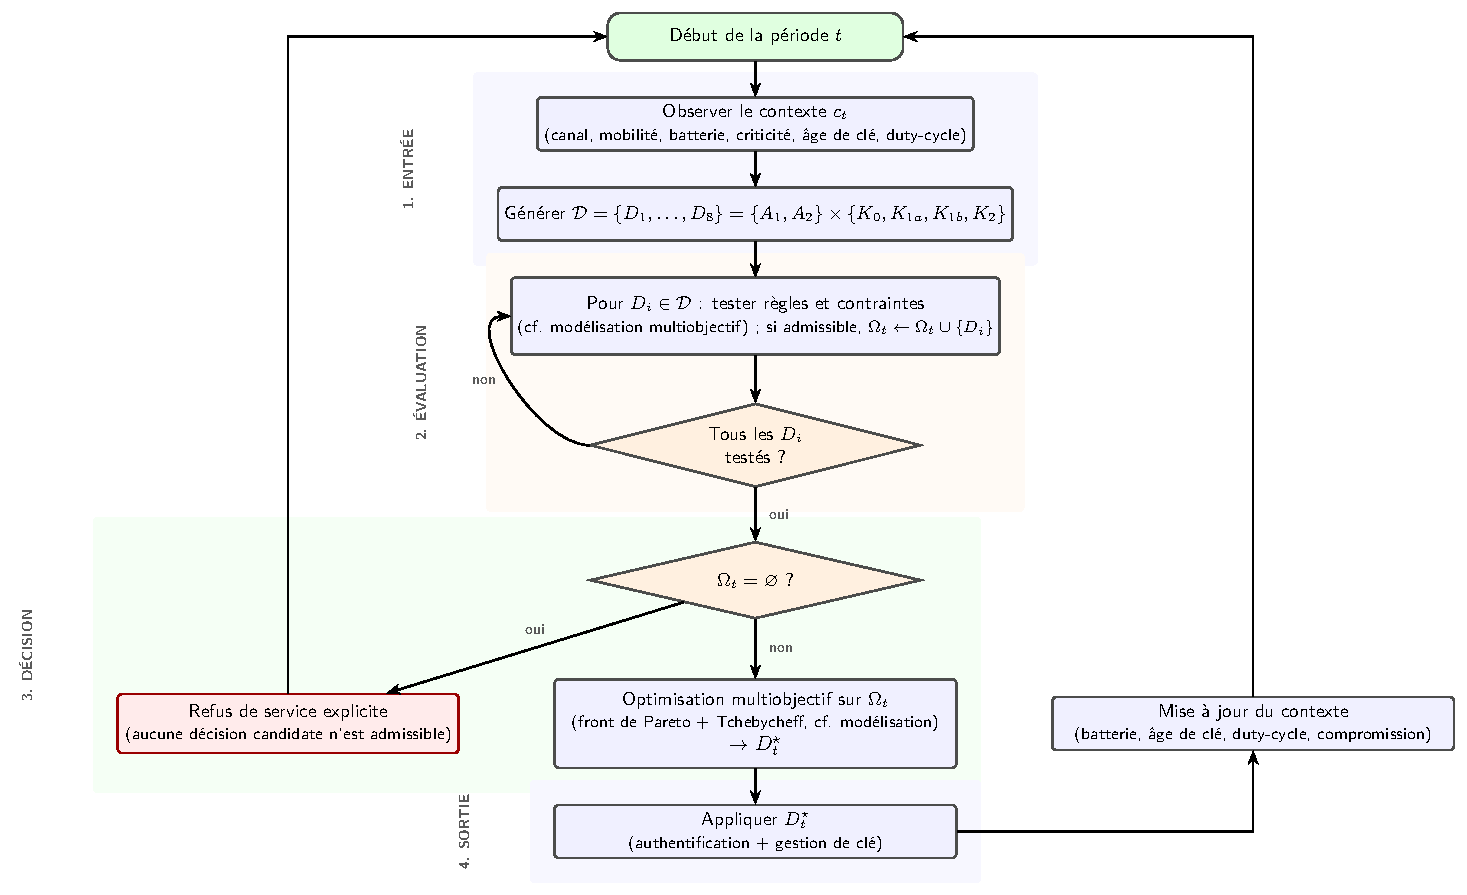
\includegraphics[width=\linewidth]{flowchart_dm.pdf}
\caption{Déroulement de la décision de P0. Le contexte est observé, les huit décisions candidates sont générées, les règles d'admissibilité sont testées, le front de Pareto est construit, puis la scalarisation de Tchebycheff sélectionne la décision appliquée.}
\label{fig:model}
\end{figure}

\section{Méthodologie}
\label{sec:methodology}

\subsection{Transposition énergétique}

L'énergie du schéma hybride est modélisée par un agrégat calibré sur les quatre points publiés. La valeur RFF seul fournit le coût de base par message $E_{\mathrm{RFF}}$. Un système linéaire $2\times2$ sur les deux points hybrides fournit deux paramètres effectifs~: un surcoût hybride fixe $F$ et un coût par repli $C$,
\begin{equation}
  E_{\mathrm{hybride}}(\mathrm{FRR}) = E_{\mathrm{RFF}} + F + N \cdot \mathrm{FRR} \cdot C,
\end{equation}
avec $N=100$ messages. Les quatre valeurs publiées sont reproduites par construction. Le paramètre $F$ n'est pas présenté comme le coût physique de l'authentification initiale, mais comme un agrégat qui peut l'absorber. La calibration est donc un ajustement sur des points publiés, et non une validation indépendante.

\subsection{Performance RFF publiée}

Lorsque P0 évalue le candidat RFF, il reçoit la performance de sécurité mesurée par Haenel et al.\ (FAR$=0{,}002$). Il ne reçoit pas le FAR d'un modèle de canal interne, qui dépend d'un rapport signal sur bruit supposé et jamais publié pour ce banc d'essai. La valeur publiée est injectée avant la scalarisation, et le FAR du candidat est composé avec la formule du moteur de décision. La variante à canal interne est conservée comme analyse de sensibilité séparée, et elle n'est jamais mélangée à la comparaison principale.

\subsection{Correction de la scalarisation}

Dans une implémentation antérieure, une petite constante numérique était ajoutée à chaque dénominateur de normalisation de la distance de Tchebycheff, y compris lorsque ce dénominateur était non dégénéré. Cela décalait les scores des candidats d'environ $2{,}5\times10^{-11}$, valeur supérieure à la tolérance utilisée pour détecter les égalités. Dans environ un tiers des périodes testées à poids égaux, le départage par FAR était ainsi contourné. La constante n'est désormais utilisée que pour détecter un écart numériquement nul. Le défaut a été identifié au cours de ce travail, puis corrigé. Tous les résultats de scénarios présentés ci-dessous proviennent de la campagne corrigée. Les résultats obtenus avec l'implémentation antérieure ne sont pas rapportés. La comparaison calibrée sur Haenel et al.\ a été calculée avec l'implémentation corrigée.

\subsection{Modèle structurel ascendant}

Un modèle énergétique événementiel TX/RX/CPU est également construit à partir des fiches techniques officielles des composants MSP430G2x et CC110L. Les paramètres non publiés (taille des trames, débit, coût de cycle de Chaskey, temps de calibration) sont variés sur des plages documentées basse, centrale et haute. Le modèle est évalué sur le surcoût incrémental au-dessus de la base RFF seul, car cette base est reproduite par construction et gonflerait sinon le pouvoir explicatif apparent du modèle.

\subsection{Scénarios expérimentaux}
\label{sec:scenarios}

Trois cadres expérimentaux sont utilisés.

\textbf{Expérience A (transposition de Haenel et al.).} Ce cadre adapte le banc d'essai énergétique de Haenel et al.~\cite{haenel2021practical}~: 300~s, 100 messages, FRR de 5\,\% et 10\,\%, deux candidats (RFF et MAC) et le FAR publié de 0,002. Seuls les deux candidats du schéma original sont conservés. Les valeurs calibrées de la section~\ref{sec:methodology} sont utilisées, et 30 graines Monte-Carlo sont simulées pour la politique de repli calibrée (B5\_HAENEL\_CALIBRATED).

\textbf{Campagne de sécurité dédiée.} Chaque politique est attaquée par 100\,000 tirages de Bernoulli. Des intervalles de confiance exacts de Clopper--Pearson à 95\,\% sont rapportés.

\textbf{Cinq scénarios adaptatifs (S1 à S5).} Ces scénarios sont définis dans le simulateur et ne sont pas repris d'une autre publication. Ils font varier le contexte de déploiement, comme le résume le tableau~\ref{tab:scenarios}. S1 est un capteur agricole isolé, à phase unique. S2 est une alarme critique industrielle, avec une phase normale, une phase d'alarme et une phase de récupération. S3 est un objet porté par un véhicule qui s'arrête, accélère, roule à 30~km/h au plus, ralentit puis s'arrête. S4 est un réseau urbain dense alternant phases normales et phases de congestion. S5 est une infrastructure critique sous attaque, avec une phase normale, une phase de compromission à forte probabilité d'attaque et une phase de récupération. Chaque scénario est simulé avec des nombres aléatoires communs entre politiques. Le nombre de graines suit une règle d'arrêt adaptative bornée entre 30 et 150 graines. Quatre politiques de référence sont comparées à P0. B1 est la politique conventionnelle, qui utilise toujours la cryptographie. B2 est une politique physique naïve, à préférence fixe et sans plancher de FAR. B3 est la règle hybride fixe, avec plancher de FAR et sans recherche de repli. B4 est le même arbitre que P0 sans plancher de FAR, et elle isole l'effet de ce plancher.

\begin{table}[t]
\centering
\caption{Configuration des cinq scénarios adaptatifs (campagne corrigée).}
\label{tab:scenarios}
\begin{tabular}{lccccc}
\toprule
 & S1 & S2 & S3 & S4 & S5 \\
\midrule
N\oe{}ud & fixe & fixe & mobile & fixe & fixe \\
RSB moyen (dB) & 8 & 6 & 9--10 & 3 & 12 \\
Probabilité d'attaque & 0,10 & 0,15 & 0,10 & 0,20--0,30 & 0,10--0,50 \\
Facteur de séparation & 4,0 & 2,0 & 2,0 & 1,0 & 0,5 \\
Profil de coût CPU & LOW & HIGH & CENTRAL & CENTRAL & HIGH \\
\bottomrule
\end{tabular}
\end{table}

\section{Résultats et discussion}
\label{sec:results}

\subsection{Comparaison calibrée sur Haenel et al.}

La figure~\ref{fig:story} compare l'énergie publiée par Haenel et al.\ avec la politique de repli calibrée et avec P0. L'énergie hybride publiée diminue lorsque le FRR baisse. La politique calibrée suit la même tendance, et sa bande de confiance à 95\,\% est représentée. P0 conserve un niveau d'énergie constant, au plafond du MAC seul, quel que soit le FRR. À poids égaux, P0 coûte donc 24,4\,\% de plus que la règle hybride à FRR=10\,\%, et 39,5\,\% de plus à FRR=5\,\%. La comparaison à FRR=5\,\% repose sur un FAR supposé, comme expliqué dans les limites ci-dessous. La figure~\ref{fig:split} présente le mélange de décisions message par message. La règle hybride mélange messages RFF et messages MAC en proportion du FRR, alors que P0 sélectionne le chemin MAC pour chaque message.

\begin{figure}[t]
\centering
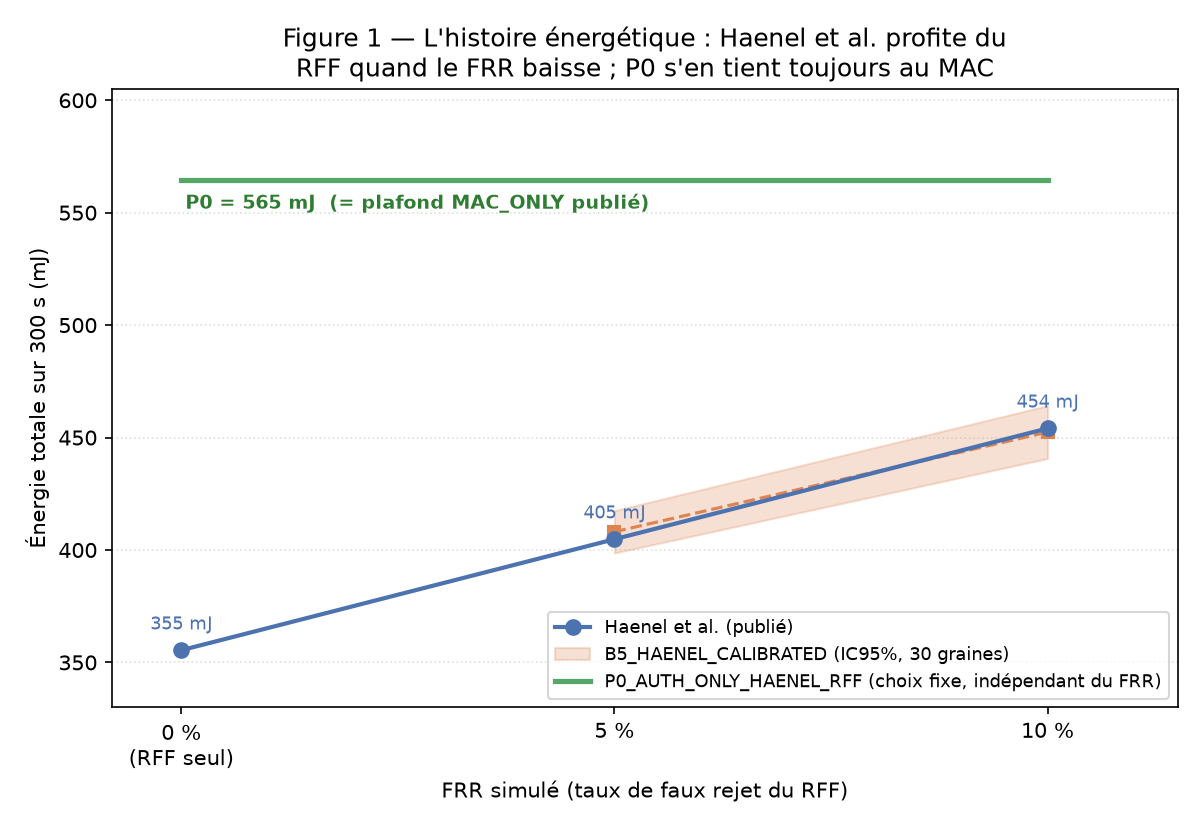
\includegraphics[width=\linewidth]{figure_1_energy_comparison.png}
\caption{Énergie calibrée en fonction du FRR simulé. La règle hybride décroît avec le FRR. P0 reste plat au plafond du MAC seul.}
\label{fig:story}
\end{figure}

\begin{figure}[t]
\centering
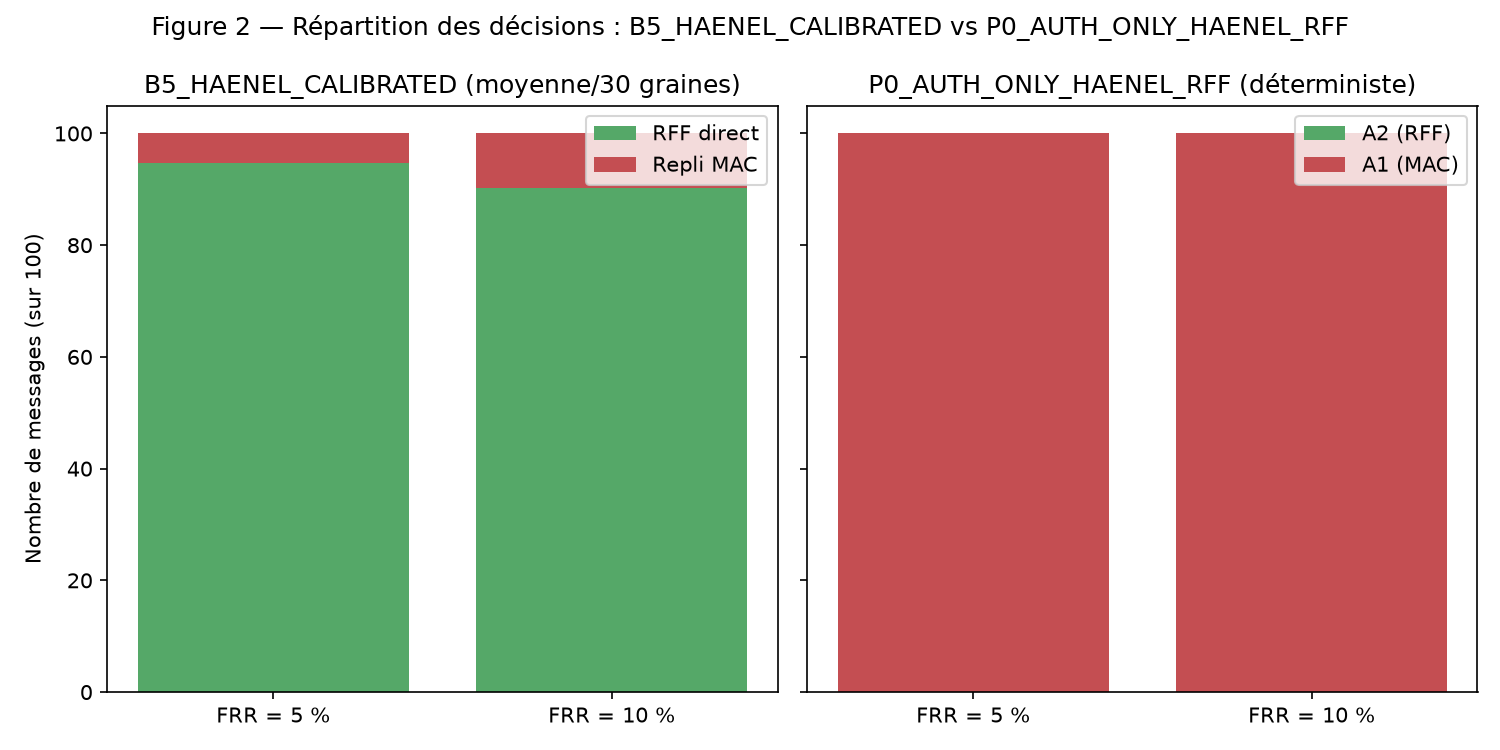
\includegraphics[width=\linewidth]{figure_2_decision_split.png}
\caption{Répartition des décisions pour 100 messages, à FRR=5\,\% et 10\,\%. La règle hybride alterne entre RFF et MAC, tandis que P0 sélectionne MAC pour tous les messages.}
\label{fig:split}
\end{figure}

\subsection{Pourquoi P0 reste sur le chemin MAC~: une égalité exacte}

La gestion de clé étant fixée et la latence neutralisée des deux côtés, le front de Pareto se réduit à deux points. Chacun est idéal sur un objectif et au nadir sur l'autre. L'équation~\eqref{eq:tcheby} se réduit alors à
\begin{equation}
  s(\text{MAC}) = w_{\mathrm{energie}}, \qquad
  s(\text{RFF}) = w_{\mathrm{auth}}.
\end{equation}
Le MAC est donc préféré lorsque $w_{\mathrm{energie}} < w_{\mathrm{auth}}$, le RFF lorsque l'inégalité est inversée, et des poids égaux donnent une égalité exacte. L'égalité est départagée par le FAR. La prédiction analytique a été vérifiée par un balayage de 11 couples de poids autour de $w_{\mathrm{energie}}=w_{\mathrm{auth}}=0{,}25$ (tableau~\ref{tab:boundary}, figure~\ref{fig:boundary}). L'écart maximal entre scores prédits et calculés est nul à la précision machine. Un déplacement de poids de 0,001 inverse la décision.

\begin{table}[t]
\centering
\caption{Balayage de la frontière des poids (cas fixé~: FRR=10\,\%, FAR=0,002).}
\label{tab:boundary}
\begin{tabular}{ccccc}
\toprule
$w_{\mathrm{energie}}$ & $w_{\mathrm{auth}}$ & $s(\mathrm{MAC})$ & $s(\mathrm{RFF})$ & Choix \\
\midrule
0,245 & 0,255 & 0,245 & 0,255 & MAC \\
0,249 & 0,251 & 0,249 & 0,251 & MAC \\
\textbf{0,250} & \textbf{0,250} & \textbf{0,250} & \textbf{0,250} & MAC (départage) \\
0,251 & 0,249 & 0,251 & 0,249 & \textbf{RFF} \\
0,255 & 0,245 & 0,255 & 0,245 & RFF \\
\bottomrule
\end{tabular}
\end{table}

\begin{figure}[t]
\centering
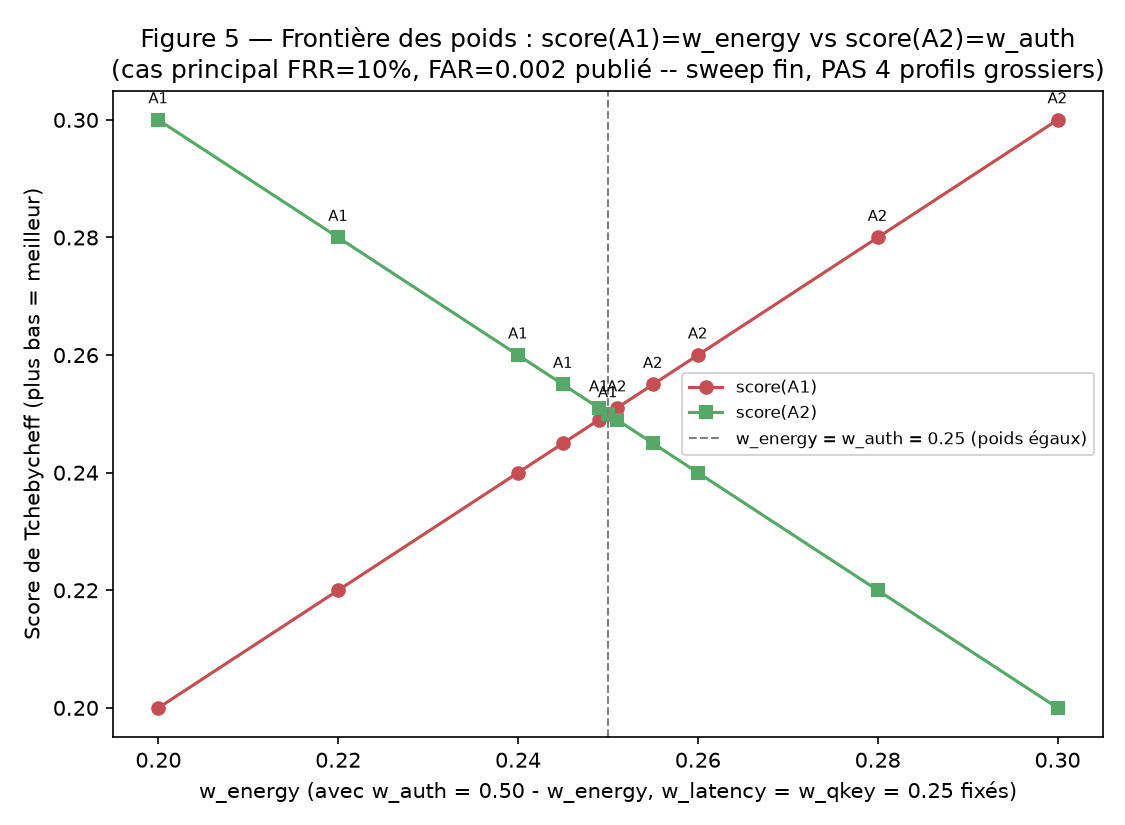
\includegraphics[width=\linewidth]{figure_5_weight_sensitivity.png}
\caption{Scores de Tchebycheff du MAC et du RFF en fonction de $w_{\mathrm{energie}}$, sur le balayage à 11 points. Les deux courbes se croisent exactement à $w_{\mathrm{energie}}=w_{\mathrm{auth}}=0{,}25$.}
\label{fig:boundary}
\end{figure}

Cette frontière est un résultat de sensibilité, et non la preuve d'une préférence forte pour la sécurité. Un lecteur qui fixe des poids légèrement différents obtient le choix RFF. Le gain énergétique du chemin RFF est réel, mais, à poids égaux, il est exactement compensé par l'avantage de robustesse du MAC.

\subsection{Campagne de sécurité}

La campagne initiale de 30 graines, avec environ 450 tentatives d'attaque, était trop petite pour estimer un FAR de 0,2\,\%. Une campagne dédiée de 100\,000 tirages par politique a donc été menée. Le chemin RFF accepte 189 tentatives sur 100\,000 (0,189\,\%, $\mathrm{IC}_{95}=[0,163\,\%,0,218\,\%]$), ce qui est cohérent avec le 0,2\,\% publié. Le chemin MAC de P0 accepte 0 tentative sur 100\,000. Sa borne supérieure à 95\,\%, $3{,}7\times10^{-5}$, est supérieure à la borne théorique du modèle, $5{,}4\times10^{-20}$. Cette campagne ne permet donc pas de distinguer les deux valeurs. Elle n'est pas présentée comme une preuve expérimentale d'une sécurité supérieure.

\begin{figure}[t]
\centering
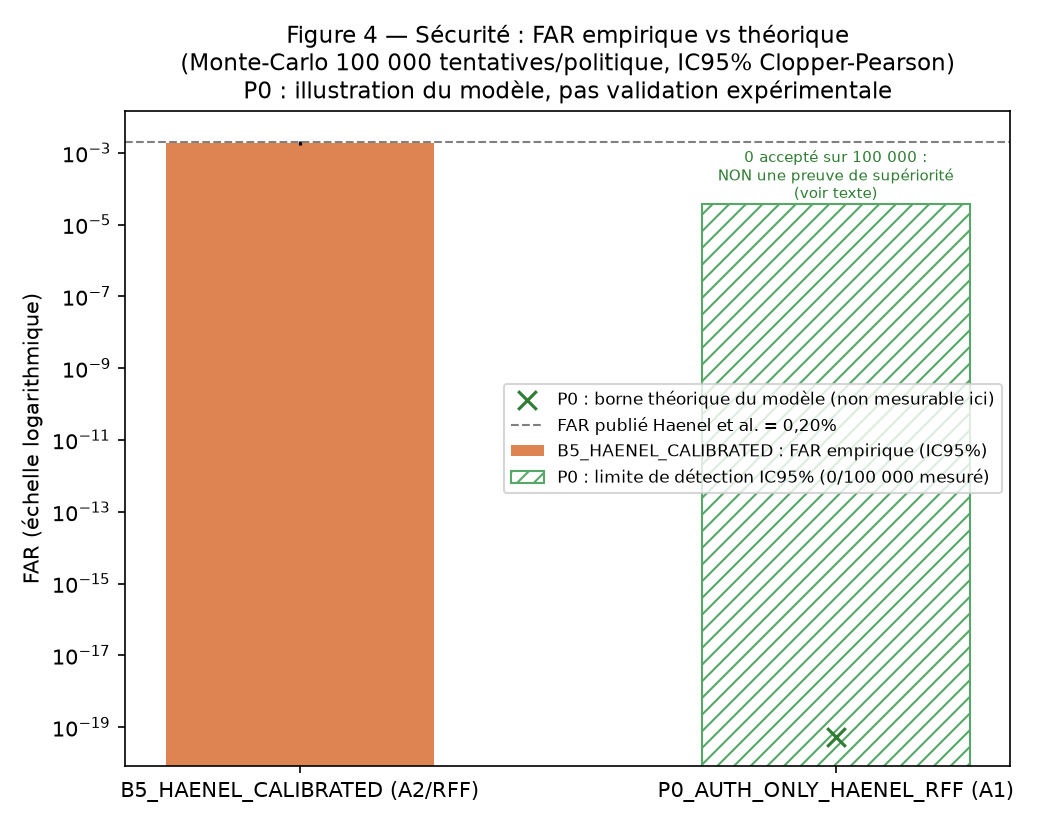
\includegraphics[width=\linewidth]{figure_4_security.png}
\caption{FAR empirique du chemin RFF, avec des intervalles de Clopper--Pearson à 95\,\%, face à la cible publiée de 0,2\,\%, et chemin MAC de P0 avec zéro acceptation sur 100\,000 tirages. La borne supérieure de l'intervalle est représentée.}
\label{fig:security}
\end{figure}

\subsection{Surcoût expliqué par le modèle ascendant}

Le surcoût incrémental du modèle ascendant, au-dessus de la base RFF seul, est comparé à la même grandeur dans les données publiées. La fraction expliquée va de 0,19\,\% (hypothèses basses) à 14,45\,\% (hypothèses hautes, cas MAC seul). L'ordre qualitatif des quatre configurations est reproduit sous chaque jeu d'hypothèses, mais pas la magnitude. Une part substantielle du surcoût réel, vraisemblablement un coût de fenêtre d'écoute ou de resynchronisation non quantifié, n'est pas expliquée par les fiches techniques publiques.

\subsection{Cinq scénarios adaptatifs}

Le tableau~\ref{tab:scen} résume la comparaison de P0 avec les politiques de référence dans la campagne corrigée. L'énergie et la latence sont moyennées sur les périodes que chaque politique sert, si bien que l'énergie d'une politique qui refuse des requêtes est calculée sur moins de périodes. Les figures~\ref{fig:s2} et~\ref{fig:s4} présentent les quatre objectifs pour les deux scénarios où les politiques de référence diffèrent le plus.

\begin{table*}[t]
\centering
\caption{Comparaison de P0 avec les politiques de référence dans les cinq scénarios (campagne corrigée ; moyennes sur les graines).}
\label{tab:scen}
\begin{tabular}{lccccc}
\toprule
 & S1 & S2 & S3 & S4 & S5 \\
\midrule
Graines & 30 & 120 & 40 & 90 & 150 \\
Tentatives de l'attaquant & 4\,426 & 26\,978 & 5\,959 & 31\,234 & 54\,131 \\
Attaques acceptées, P0 (nombre) & 0 & 0 & 0 & 0 & 0 \\
Attaques acceptées, B2 (\%) & 0 & 12,6 & 1,1 & 70,6 & 55,2 \\
Attaques acceptées, B3 (\%) & 0 & 0,4 & 0,1 & 0,04 & 0 \\
Économie d'énergie vs B1 (\%) & 2,8 & 0,08 & 0,02 & 0,02 & 6,9 \\
Surcoût d'énergie vs B2 (\%) & 2,1 & 3,9 & 4,8 & 4,8 & 4,1 \\
Latence, P0 / B1 (objectif) & 0,0015 / 0,0019 & 0,0050 / 0,0050 & 0,0019 / 0,0019 & 0,0020 / 0,0019 & 0,053 / 0,0035 \\
Qualité de clé, P0 / B1 & 0,730 / 0,731 & 0,730 / 0,731 & 0,731 / 0,731 & 0,731 / 0,731 & 0,669 / 0,745 \\
Taux de service, P0 (\%) & 100 & 100 & 100 & 100 & 100 \\
Taux de service, B1 (\%) & 100 & 100 & 100 & 100 & 94,8 \\
Taux de service, B3 (\%) & 99,99 & 38,8 & 44,1 & 2,5 & 0,05 \\
\bottomrule
\end{tabular}
\end{table*}

\begin{figure}[t]
\centering
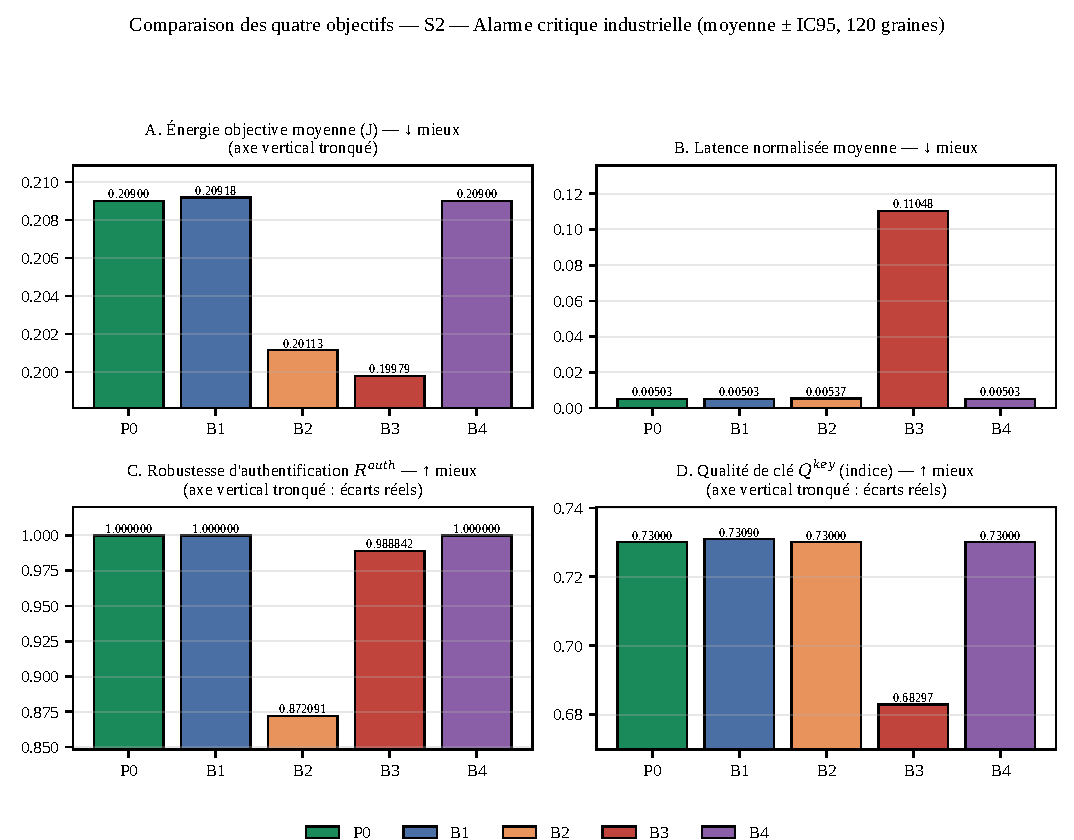
\includegraphics[width=\linewidth]{figure_s2_four_objectives.pdf}
\caption{Quatre objectifs pour S2 (alarme critique industrielle, 120 graines). B2 accepte 12,6\,\% des tentatives de l'attaquant, contre aucune pour P0. B3 sert 38,8\,\% des requêtes.}
\label{fig:s2}
\end{figure}

\begin{figure}[t]
\centering
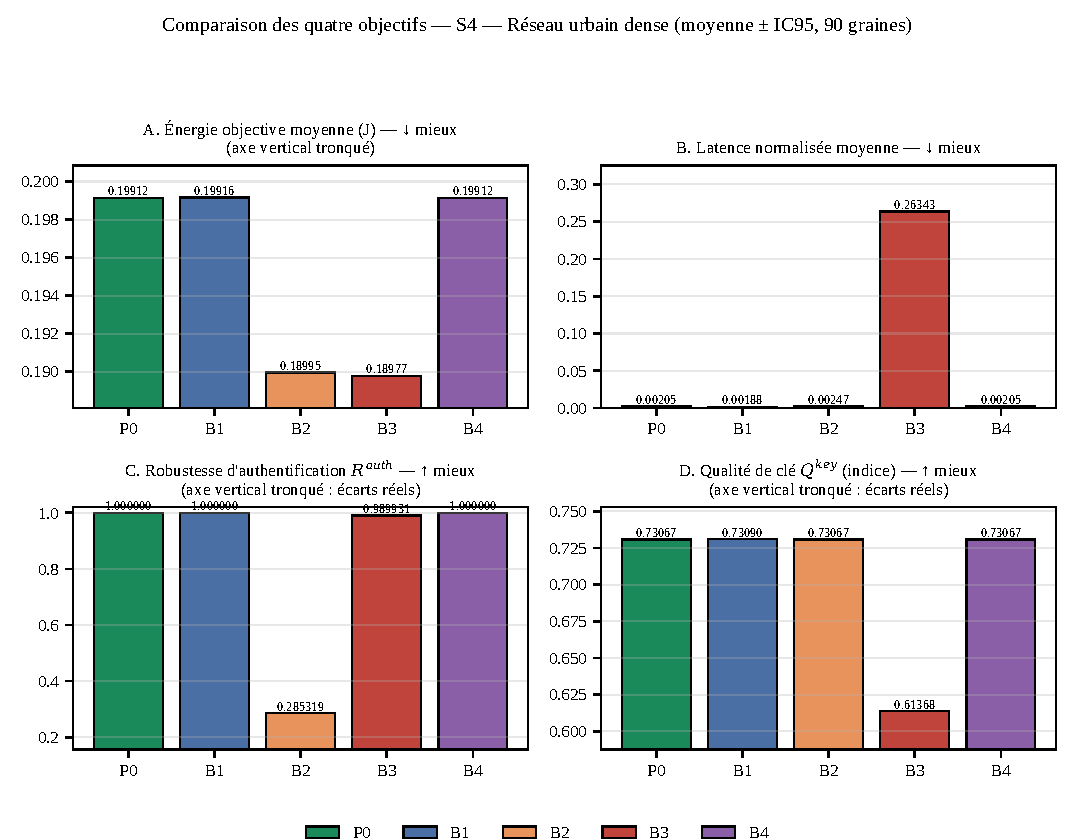
\includegraphics[width=\linewidth]{figure_s4_four_objectives.pdf}
\caption{Quatre objectifs pour S4 (réseau urbain dense, 90 graines). B2 accepte 70,6\,\% des tentatives de l'attaquant, avec une robustesse de 0,285. B3 sert 2,5\,\% des requêtes.}
\label{fig:s4}
\end{figure}

\subsection{Les cas où P0 fait mieux, et ceux où il ne fait pas mieux}

P0 n'accepte aucune attaque dans les cinq scénarios, et il ne refuse aucune requête. Son nombre d'acceptations est nul sur 4\,426 à 54\,131 tentatives, de sorte que sa borne supérieure à 95\,\% vaut environ $3/N$, soit au plus $5{,}5\times10^{-5}$ pour S5. La politique physique naïve B2 accepte entre 1,1\,\% et 70,6\,\% des attaques en S2 à S5, et sa robustesse tombe à 0,285 en S4. La règle hybride fixe B3 ne sert que 2,5\,\% des requêtes en S4 et 0,05\,\% en S5. Face à la politique conventionnelle B1, P0 économise 2,8\,\% d'énergie en S1 et 6,9\,\% en S5. En S5, B1 refuse 5,2\,\% des requêtes, si bien que sa moyenne d'énergie porte sur moins de périodes et n'est pas strictement comparable.

P0 ne fait pas mieux sur tous les critères. Son énergie est supérieure de 2,1\,\% à 4,8\,\% à celle de B2, qui accepte les attaques sans restriction. En S4, la latence de P0 est supérieure de 9\,\% à celle de B1. En S5, P0 présente une latence de 0,053 contre 0,0035 pour B1, et une qualité de clé de 0,669 contre 0,745. Dans ce scénario, P0 partage ces pénalités avec B2, qui a la même latence et la même qualité de clé. L'économie d'énergie face à B1 en S2 à S4 est inférieure à 0,1\,\%. Elle est statistiquement distinguable de zéro dans l'analyse appariée, mais elle est trop faible pour avoir un effet pratique.

\subsection{Limites}

Plusieurs limites encadrent ces résultats. Les valeurs d'énergie proviennent d'un modèle calibré, et les paramètres CPU attendent encore une mesure matérielle. L'énergie moyenne varie d'environ 8\,\% entre les profils de paramètres CPU bas et haut. Cette variation ne suffit pas à inverser les comparaisons qualitatives, mais elle affecte les pourcentages rapportés ci-dessus. Le canal est simulé, et aucune mesure radio n'est utilisée. Les poids de P0 sont égaux par construction, et aucun jeu de poids contextuel n'a été validé. La campagne S5 n'a pas atteint la précision préenregistrée dans sa limite de 150 graines. L'analyse à deux candidats de l'expérience A est un cas réduit, et ses conclusions sur la frontière de décision ne se transposent pas directement au cadre à cinq scénarios.

\section{Conclusion}

Un arbitre de décision multiobjectif est comparé à une règle de repli fixe et à trois autres politiques, sous des planchers de sécurité explicites. Dans la campagne corrigée, P0 n'accepte aucune attaque et sert toutes les requêtes dans les cinq scénarios. Il n'économise de l'énergie face à la cryptographie conventionnelle qu'en S1 et S5. Il paie un surcoût énergétique modéré face à une politique physique naïve qui accepte des attaques, ainsi qu'une pénalité de latence et de qualité de clé en S5. Dans le cas réduit calibré sur Haenel et al., la décision à poids égaux se situe sur une égalité exacte. Les travaux futurs incluent la mesure des paramètres CPU et radio sur matériel, la validation d'un jeu de poids contextuel et l'extension de la comparaison à des canaux dynamiques.

\section{Implémentation}

Le simulateur, les scripts de calibration, la suite de tests et les instructions permettant de régénérer chaque figure et chaque tableau sont disponibles à l'adresse \url{https://github.com/guygnyolparfait/physec-dm-p0-haenel}. Le dépôt reste privé pendant la préparation et sera rendu public à la fin du travail.

\begin{thebibliography}{11}

\bibitem{haenel2021practical}
A.~Haenel, Y.~Haddad, M.~Laurent et Z.~Zhang, ``Practical cross-layer radio frequency-based authentication scheme for internet of things,'' \emph{Sensors}, vol.~21, no.~12, p.~4034, 2021.

\bibitem{das2018deep}
R.~Das, A.~Gadre, S.~Zhang, S.~Kumar et J.~M.~F. Moura, ``A deep learning approach to IoT authentication,'' dans \emph{Proc. IEEE Int. Conf. Communications (ICC)}, 2018.

\bibitem{baldini2017physical}
G.~Baldini, R.~Giuliani, G.~Steri et R.~Neisse, ``Physical layer authentication of Internet of Things wireless devices through permutation and dispersion entropy,'' dans \emph{Proc. IEEE Global Internet of Things Summit (GIoTS)}, 2017.

\bibitem{nouichi2019iot}
D.~Nouichi, M.~Abdelsalam, Q.~Nasir et S.~Abbas, ``IoT devices security using RF fingerprinting,'' dans \emph{Proc. IEEE Int. Conf. Advances in Science and Engineering Technology (ASET)}, 2019.

\bibitem{merchant2019enhanced}
K.~Merchant et B.~Nousain, ``Enhanced RF fingerprinting for IoT devices with recurrent neural networks,'' dans \emph{Proc. IEEE Military Communications Conf. (MILCOM)}, 2019, pp.~590--597.

\bibitem{wilson2019integration}
A.~J. Wilson, D.~R. Reising et T.~D. Loveless, ``Integration of matched filtering within the RF-DNA fingerprinting process,'' dans \emph{Proc. IEEE Global Communications Conf. (GLOBECOM)}, 2019.

\bibitem{gopalakrishnan2019robust}
S.~Gopalakrishnan, M.~Cekic et U.~Madhow, ``Robust wireless fingerprinting via complex-valued neural networks,'' présenté à \emph{IEEE Global Communications Conf. (GLOBECOM)}, 2019. [En ligne]. Disponible~: arXiv:1905.09388.

\bibitem{morge2022rf}
L.~Morge-Rollet, F.~Le~Roy, D.~Le~Jeune, C.~Canaff et R.~Gautier, ``RF eigenfingerprints, an efficient RF fingerprinting method in IoT context,'' \emph{Sensors}, vol.~22, no.~11, p.~4291, 2022.

\bibitem{li2018robust}
X.~Li, J.~Peng, J.~Niu, F.~Wu, J.~Liao et K.-K.~R. Choo, ``A robust and energy efficient authentication protocol for industrial internet of things,'' \emph{IEEE Internet of Things Journal}, vol.~5, no.~3, pp.~1606--1615, 2018.

\bibitem{prantl2023recommendation}
T.~Prantl, A.~Bauer, L.~Iffl\"ander, C.~Krupitzer et S.~Kounev, ``Recommendation of secure group communication schemes using multi-objective optimization,'' \emph{Int. J. Information Security}, vol.~22, no.~5, pp.~1291--1332, 2023.

\bibitem{prvulovic2025hermees}
P.~Prvulovic, N.~Radosavljevic, D.~Babic et D.~Drajic, ``HERMEES: A holistic evaluation and ranking model for energy-efficient systems applied to selecting optimal lightweight cryptographic and topology construction protocols in wireless sensor networks,'' \emph{Sensors}, vol.~25, no.~9, p.~2732, 2025.

\end{thebibliography}

\end{document}
